        	\begin{question}{1206}{Vecteurs}{1}{1217}
				Soit $\vec{A}=(a_x;a_y)$ un vecteur. Quel est le lien entre sa norme, sa composante sur $x$ et l'angle $\theta$ entre $\vec{A}$ et l'axe $x$?
            \end{question}
            \begin{reponses}
            	\item[true] $\cos(\theta)=\frac{a_x}{||\vec{A}||}$
            	\item[false] $\sin(\theta)=\frac{a_x}{||\vec{A}||}$
                \item[false] $\cos(\theta)=\frac{||\vec{A}||}{a_x}$
                \item[false] $\sin(\theta)=\frac{||\vec{A}||}{a_x}$
            \end{reponses}
			%%%%%%%%%%%%%%%%%%%%%%%%%%%%%%%%%%%%%
        	\begin{question}{1206}{Vecteurs}{1}{1217}
				Soit $\vec{A}=(a_x;a_y)$ un vecteur. Quel est le lien entre sa norme, sa composante sur $y$ et l'angle $\theta$ entre $\vec{A}$ et l'axe $x$?
            \end{question}
            \begin{reponses}
            	\item[false] $\cos(\theta)=\frac{a_y}{||\vec{A}||}$
            	\item[true] $\sin(\theta)=\frac{a_y}{||\vec{A}||}$
                \item[false] $\cos(\theta)=\frac{||\vec{A}||}{a_y}$
                \item[false] $\sin(\theta)=\frac{||\vec{A}||}{a_y}$
            \end{reponses}
			%%%%%%%%%%%%%%%%%%%%%%%%%%%%%%%%%%%%%
            \begin{question}{1206}{Vecteurs}{2}{1217}
                Quelles sont les composantes du vecteur $\vec{AB}$?\\
                \begin{center}
                	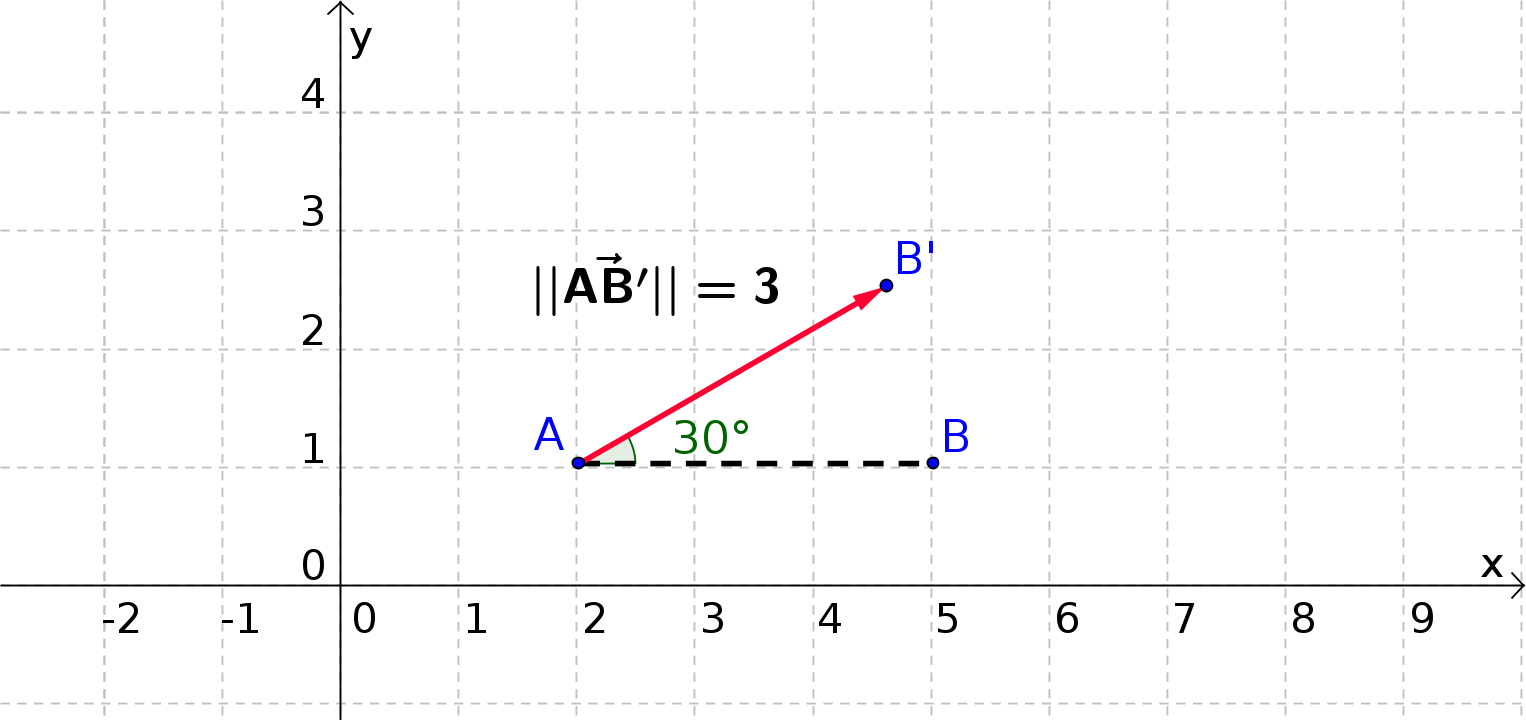
\includegraphics[width=0.5\textwidth]{Philippe/Figures_Philippe/vecteurs_4_6.png}
                \end{center}
            \end{question}
            \begin{reponses}
                \item[false] $(5;2.5)$
                \item[false] $(3;1)$
                \item[false] $(3;1,5)$
                \item[true] $(3\sqrt{3}/2;1,5)$
            \end{reponses}
            %%%%%%%%%%%%%%%%%%%%%%%%%%%%%%%%%%%%%
        	\begin{question}{1206}{Vecteurs}{2}{1217}
				Soit $\vec{A}$ un vecteur de norme $||\vec{A}||$ faisant un angle $\theta$ avec l'axe des $x$. Quelle est sa coordonnée selon $x$?
            \end{question}
            \begin{reponses}
            	\item[true] $||\vec{A}||\cos(\theta)$
            	\item[false] $||\vec{A}||\sin(\theta)$
                \item[false] $||\vec{A}||\tan(\theta)$
                \item[false] $||\vec{A}||/2$
            \end{reponses}
			%%%%%%%%%%%%%%%%%%%%%%%%%%%%%%%%%%%%%
        	\begin{question}{1206}{Vecteurs}{2}{1217}
				Soit $\vec{A}$ un vecteur de norme $||\vec{A}||$ faisant un angle $\theta$ avec l'axe des $x$. Quelle est sa coordonnée selon $y$?
            \end{question}
            \begin{reponses}
            	\item[false] $||\vec{A}||\cos(\theta)$
            	\item[true] $||\vec{A}||\sin(\theta)$
                \item[false] $||\vec{A}||\tan(\theta)$
                \item[false] $||\vec{A}||/2$
            \end{reponses}
			%%%%%%%%%%%%%%%%%%%%%%%%%%%%%%%%%%%%%
